%============================================================
% BAB 4: RANCANGAN DAN IMPLEMENTASI SISTEM
%============================================================
\chapter{RANCANGAN DAN IMPLEMENTASI SISTEM}

Bab ini menguraikan proses perancangan dan implementasi teknis sistem perangkat lunak yang dikerjakan selama pelaksanaan kerja praktik di \NamaPerusahaan\ dalam periode \PeriodeKP. Pembahasan diawali dengan standarisasi pengembangan perangkat lunak yang berlaku di perusahaan, diikuti oleh pembahasan mendalam mengenai rancangan dan realisasi teknis proyek utama pertama, yaitu \textbf{Proyek MonGrid}. Bagian akhir bab menyajikan kerangka kerja untuk proyek-proyek berikutnya serta skema pengujian dan evaluasi fungsional.

\section{STANDAR PENGEMBANGAN PERUSAHAAN}

Sebagai bagian dari tim rekayasa perangkat lunak di \NamaPerusahaan, penulis diwajibkan mematuhi pedoman dan konvensi pengembangan yang terstandarisasi. Penerapan standar ini bertujuan menjamin keterbacaan kode, konsistensi antar-layanan, efisiensi peninjauan kode, serta keandalan proses integrasi berkelanjutan (\textit{Continuous Integration}).

\subsection{Konvensi Version Control dan \textit{Conventional Commits}}

Pengelolaan kode sumber pada seluruh repositori di lingkungan PT. Sinergi Dimensi Informatika memanfaatkan sistem kendali versi Git dengan platform GitLab. Penulisan pesan komit (\textit{commit message}) wajib mengikuti spesifikasi \textit{Conventional Commits} yang dipadukan dengan kode penanda untuk mempercepat identifikasi visual pada riwayat perubahan repositori. Format standar pesan komit didefinisikan sebagai berikut:

\begin{center}
  \texttt{<type>(<scope>): <deskripsi singkat>}
\end{center}

Rincian klasifikasi tipe komit, contoh format penggunaan, serta skenario penerapannya dirangkum pada Tabel~\ref{tab:commit_types}.

\begin{longtblr}[
  caption = {Standarisasi Tipe Komit Git di PT. Sinergi Dimensi Informatika},
  label = {tab:commit_types}
]{
  colspec = {Q[c,m,1.2cm] Q[l,m,3.6cm] Q[l,m,5.0cm]},
  hlines,
  vlines,
  row{1} = {font=\bfseries, halign=c},
}
  Tipe & Contoh Format & Kapan Digunakan \\
  \texttt{feat} & \texttt{feat(alarm): add redis log} & Penambahan fitur atau kapabilitas baru \\
  \texttt{fix} & \texttt{fix(ingest): handle null meter} & Perbaikan kesalahan program (\textit{bug}) \\
  \texttt{perf} & \texttt{perf(sync): batch redis scan} & Peningkatan performa dan optimasi latensi \\
  \texttt{refactor} & \texttt{refactor(handler): split logic} & Restrukturisasi kode tanpa mengubah fungsionalitas \\
  \texttt{docs} & \texttt{docs(readme): update topology} & Pembaruan dokumentasi teknis atau berkas README \\
  \texttt{test} & \texttt{test(consumer): add unit test} & Penambahan atau modifikasi pengujian unit \\
  \texttt{chore} & \texttt{chore: update package references} & Pemeliharaan rutin dependensi, konfigurasi, atau CI \\
  \texttt{remove} & \texttt{remove(legacy): drop unused dto} & Penghapusan berkas atau kode yang sudah usang \\
  \texttt{security} & \texttt{security(auth): sanitize tokens} & Mitigasi kerentanan keamanan atau proteksi data \\
\end{longtblr}

Penerapan aturan komit tersebut mewajibkan pesan komit bersifat atomik (satu komit berfokus pada satu perubahan logis), menggunakan kata kerja imperatif berbahasa Inggris, mendefinisikan modul atau sub-layanan terkait pada bagian cakupan (\textit{scope}), serta membatasi panjang baris subjek maksimal 72 karakter.

\subsection{Tata Kelola Peninjauan Kode dan \textit{Merge Request}}

Setiap penambahan atau pembaruan kode tidak diperkenankan langsung digabungkan ke cabang utama (\texttt{main}). Alur kerja yang diterapkan mengadopsi model percabangan berbasis fitur (\textit{feature branching}):

\begin{enumerate}[label=\arabic*., leftmargin=*, itemsep=0pt]
  \item \textbf{Pembuatan Cabang Fitur:} Pengembang membuat cabang baru dari cabang \texttt{main} dengan format penamaan terstruktur, seperti \texttt{feat/<nama-fitur>} atau \texttt{fix/<nama-masalah>}.
  \item \textbf{Verifikasi Otomatis (\textit{Automated Pipeline}):} Setiap \textit{push} memicu proses kompilasi otomatis, pemeriksaan analisis statis (\textit{linter}), dan pengujian unit pada GitLab CI/CD.
  \item \textbf{Pengajuan \textit{Merge Request} (MR):} Pengembang menyusun deskripsi MR yang mencantumkan ringkasan perubahan teknis, dampak sistem, serta bukti pengujian mandiri.
  \item \textbf{Peninjauan Sejawat (\textit{Peer Review}):} Kode ditinjau minimal oleh satu pengembang senior atau rekan tim untuk memverifikasi kesesuaian arsitektur, kepatuhan konvensi penamaan, dan potensi regresi sebelum disetujui (\textit{approved}) dan digabungkan.
\end{enumerate}

\subsection{Standar Arsitektur Perangkat Lunak}

Untuk menjaga pemisahan tanggung jawab (\textit{Separation of Concerns}) dan kemudahan perawatan dalam jangka panjang, pengembangan layanan di PT. Sinergi Dimensi Informatika menerapkan standar arsitektur berlapis:

\begin{itemize}[leftmargin=*, itemsep=0pt]
  \item \textbf{Layanan \textit{Backend} (.NET):} Mengikuti pola \textit{Clean Architecture} dengan dependensi mengarah ke dalam. Lapisan terdiri dari \texttt{Domain} (entitas inti), \texttt{Application} (antarmuka, DTO, logika bisnis), \texttt{Infrastructure} (akses data EF Core, klien Redis/RabbitMQ/InfluxDB), dan \texttt{API} (\textit{controller} dan \textit{middleware}).
  \item \textbf{Layanan \textit{Frontend} (React):} Mengikuti struktur modular berbasis fitur (\textit{feature-based structure}) dengan pemisahan tegas antara komponen presentasi (\textit{primitives} dan UI), manajemen \textit{server state} (TanStack Query), \textit{client state} (Zustand), serta lapisan integrasi API/WebSocket terpusat.
\end{itemize}

\subsection{Pengelolaan Konfigurasi dan Keamanan Kredensial}

Konfigurasi aplikasi dikelola secara terpusat dengan memisahkan kode sumber dari data sensitif:
\begin{itemize}[leftmargin=*, itemsep=0pt]
  \item Berkas \texttt{appsettings.json} atau \texttt{.env} hanya memuat konfigurasi generik dan templat variabel.
  \item Kredensial rahasia (\textit{secrets}), seperti kata sandi basis data, kunci API, dan token koneksi \textit{message broker}, diinjeksikan melalui variabel lingkungan (\textit{environment variables}) kontainer atau penyedia brankas rahasia (\textit{Secret Manager} HashiCorp Vault), sehingga tidak pernah tersimpan di repositori Git.
\end{itemize}

%============================================================
\section{PROYEK MONGRID}
%============================================================

Proyek MonGrid adalah platform pemantauan dan analisis kondisi teknis jaringan distribusi tenaga listrik yang dikembangkan untuk mendukung pemantauan terpusat dan preventif pada gardu distribusi, transformator tenaga, panel hubung bagi, dan kubikel. 

\subsection{Gambaran Umum dan Kebutuhan Sistem}

Pada sistem konvensional, pemeriksaan kondisi peralatan gardu listrik sering kali bergantung pada inspeksi fisik manual secara berkala atau respons darurat ketika telah terjadi pemadaman listrik akibat kerusakan peralatan. Ketiadaan data operasional langsung (\textit{real-time}) menghambat deteksi dini terhadap fenomena degradasi aset, seperti ketidakseimbangan beban antarfasa, arus netral yang berlebihan, lonjakan temperatur belitan trafo, atau penurunan kualitas daya.

MonGrid hadir untuk menjembatani kesenjangan tersebut melalui digitalisasi menyeluruh. Sistem ini mengumpulkan telemetri berkecepatan tinggi dari ribuan titik sensor lapangan, melakukan normalisasi dan kalkulasi nilai rekayasa turunan secara otomatis, mendeteksi anomali ambang batas alarm dalam hitungan detik, serta menyajikan dasbor pemantauan multi-skala yang interaktif bagi operator dan manajer operasional.

Untuk mewujudkan kapabilitas tersebut, sistem MonGrid menuntut integrasi rekayasa perangkat lunak yang andal dengan kebutuhan fungsional dan teknis utama sebagai berikut:
\begin{enumerate}[label=\alph*., leftmargin=*, itemsep=0pt]
  \item \textbf{Dukungan Telemetri Frekuensi Tinggi:} Kemampuan menyerap aliran data sensor yang tiba setiap detik tanpa kehilangan paket data atau mengalami penurunan kinerja (\textit{zero packet loss}).
  \item \textbf{Pemrosesan Nilai Turunan Instan:} Kalkulasi nilai-nilai rekayasa kelistrikan yang tidak dikirimkan langsung oleh perangkat meter fisik, seperti arus netral fasa, persentase ketidakseimbangan beban, dan persentase kapasitas trafo.
  \item \textbf{Evaluasi Aturan Alarm Dinamis:} Evaluasi kondisi telemetri terhadap aturan ambang batas (\textit{threshold}) yang dapat dikonfigurasi secara fleksibel oleh administrator tanpa perlu melakukan kompilasi ulang kode sumber.
  \item \textbf{Sinkronisasi Multi-Penyimpanan (\textit{Polyglot Persistence}):} Penyelarasan data terpadu antara basis data relasional (PostgreSQL), basis data memori berkecepatan tinggi (Redis), dan basis data deret waktu (\textit{time-series} InfluxDB).
  \item \textbf{Penyajian Real-Time Dual-Channel pada Dasbor Web:} Antarmuka pengguna yang mampu memadukan pemuatan data historis terpaginasi via REST API dengan pembaruan status telemetri dan peringatan alarm seketika via WebSocket STOMP tanpa jeda penyegaran manual (\textit{no polling}).
\end{enumerate}

Sesuai ruang lingkup penugasan kerja praktik, pembahasan teknis pada proyek MonGrid difokuskan pada perancangan dan implementasi arsitektur \textit{backend} dan \textit{data pipeline} serta perancangan dan integrasi antarmuka \textit{frontend} pemantauan terpusat. Komponen aplikasi bergerak (\textit{mobile}) berada di luar lingkup kerja dan tanggung jawab penulis sehingga tidak dibahas dalam laporan ini.

\subsection{Rancangan Arsitektur Sistem dan Alur Data}

MonGrid mengadopsi arsitektur terdistribusi berbasis layanan (\textit{service-oriented}) yang memadukan pola komunikasi asinkron berbasis pesan (\textit{Publish-Subscribe}) untuk pemrosesan telemetri berkecepatan tinggi dengan pola sinkron REST API untuk manajemen data master dan penyajian kueri.

\begin{figure}[H]
  \centering
  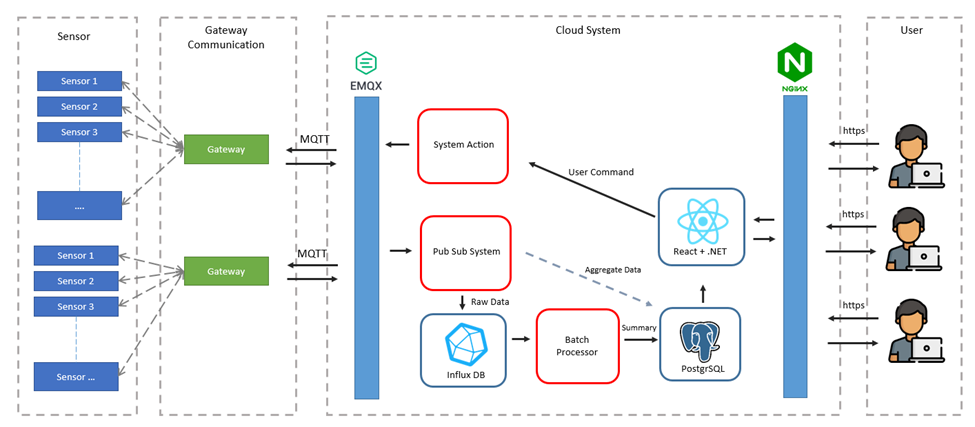
\includegraphics[width=\textwidth]{assets/gambar/mongrid/desain-arsitektur-teknis.png}
  \caption{Realisasi Teknis Arsitektur Sistem MonGrid}
  \label{fig:mongrid_arsitektur_teknis}
\end{figure}

Berdasarkan rancangan teknis pada Gambar~\ref{fig:mongrid_arsitektur_teknis}, arsitektur MonGrid membagi alur data ke dalam lima lapisan logis fungsional:
\begin{enumerate}[label=\arabic*., leftmargin=*, itemsep=0pt]
  \item \textbf{Lapisan Perangkat Lapangan (\textit{Edge Layer}):} Perangkat meter pintar (\textit{Power Meter}) dan sensor temperatur/kelembaban yang terpasang pada gardu membaca besaran listrik, lalu mempublikasikan data mentah secara periodik melalui protokol MQTT dengan jaminan pengiriman QoS 1 ke broker perantara.
  \item \textbf{Lapisan Akuisisi (\textit{Ingestion Broker}):} Broker MQTT \textbf{EMQX} bertindak sebagai gerbang terdepan penampung koneksi IoT lapangan skala besar.
  \item \textbf{Lapisan Pemrosesan Data (\textit{Processing Pipeline}):}
  \begin{itemize}[leftmargin=*, itemsep=0pt]
    \item \textbf{Mongrid Producer:} Layanan tanpa kepala (\textit{headless .NET service}) yang berlangganan topik MQTT, melakukan validasi struktur pesan, menyaring tipe paket, dan meneruskannya ke antrean pesan internal.
    \item \textbf{RabbitMQ Broker:} Berperan sebagai penyangga durabel (\textit{durable buffer}) untuk menyerap lonjakan data (\textit{burst traffic}) dan mengisolasi lapisan penerimaan dari lapisan kalkulasi.
    \item \textbf{Mongrid Consumer:} Mesin komputasi telemetri yang mengonsumsi antrean RabbitMQ, memetakan kode parameter meter, menghitung nilai rekayasa turunan, mengevaluasi aturan alarm, serta mendistribusikan data ke penyimpanan.
  \end{itemize}
  \item \textbf{Lapisan Penyimpanan (\textit{Polyglot Persistence}):}
  \begin{itemize}[leftmargin=*, itemsep=0pt]
    \item \textbf{Redis (In-Memory Cache):} Menyimpan status telemetri terkini (\textit{latest device state}), status alarm aktif, serta *cache* konfigurasi pemetaan perangkat.
    \item \textbf{InfluxDB (Time-Series Database):} Menyimpan deret waktu data pengukuran mentah dan teragregasi untuk kebutuhan analisis tren historis.
    \item \textbf{PostgreSQL (Relational Database):} Menyimpan data master hierarki aset gardu, konfigurasi akun pengguna, aturan batas alarm, log kejadian, dan tiket insiden.
  \end{itemize}
  \item \textbf{Lapisan Orkestrator dan Penyajian (\textit{Sync \& Presentation Layer}):}
  \begin{itemize}[leftmargin=*, itemsep=0pt]
    \item \textbf{Mongrid Background Service (BgService):} Layanan latar belakang yang melakukan sinkronisasi data master dari PostgreSQL ke Redis, mem-\textit{flush} data telemetri mutakhir dari Redis ke PostgreSQL, serta memancarkan siaran (\textit{blast}) alarm ke kanal STOMP RabbitMQ.
    \item \textbf{Mongrid Backend API:} Layanan REST API berbasis \textit{Clean Architecture} (.NET 9) yang melayani kueri data master, autentikasi pengguna, manajemen tiket, dan kueri pelaporan.
    \item \textbf{Mongrid Frontend:} Aplikasi web dasbor pemantauan interaktif (React 19 + TypeScript) yang mengonsumsi REST API dan berlangganan STOMP over WebSocket.
  \end{itemize}
\end{enumerate}

\begin{figure}[H]
  \centering
  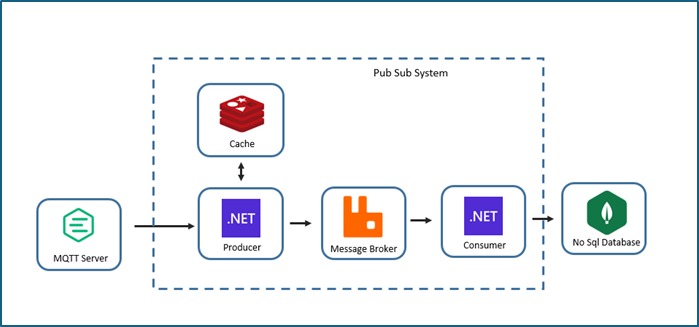
\includegraphics[width=0.88\textwidth]{assets/gambar/mongrid/pub-sub-system.png}
  \caption{Pola \textit{Publish-Subscribe} Pemrosesan Data Telemetri MonGrid}
  \label{fig:mongrid_pubsub}
\end{figure}

Pemisahan tanggung jawab antara produsen pesan (\textit{Producer}), antrean pesan (\textit{RabbitMQ}), dan konsumen pemroses (\textit{Consumer}) sebagaimana diilustrasikan pada Gambar~\ref{fig:mongrid_pubsub} merupakan keputusan arsitektural krusial. Pola ini memastikan bahwa proses komputasi yang berat dan operasi penyimpanan tidak pernah memblokir penerimaan telemetri sensor di gerbang depan, serta memungkinkan penskalaan horizontal (\textit{horizontal scaling}) pada setiap komponen secara independen.

\subsection{Implementasi Pipeline Ingesti dan Pemrosesan Telemetri}

Alur kerja ingesti data telemetri MonGrid dirancang dengan memecah fungsionalitas ke dalam dua komponen utama: \texttt{mongrid-producer} dan \texttt{mongrid-consumer}.

\subsubsection{Mongrid Producer (MQTT-to-AMQP Ingestion Bridge)}

Layanan \texttt{mongrid-producer} dikembangkan menggunakan .NET 9 berbasis \textit{Generic Host}. Layanan ini berfungsi sebagai jembatan protokol (\textit{protocol bridge}) yang sengaja dirancang ramping (\textit{deliberately thin}), tanpa koneksi ke basis data relasional.

Alasan teknis pemisahan \textit{Producer} di gerbang awal mencakup:
\begin{itemize}[leftmargin=*, itemsep=0pt]
  \item \textbf{Penerjemahan Protokol:} Perangkat lapangan berkomunikasi via MQTT, sementara ekosistem internal MonGrid berkomunikasi via AMQP. Producer memusatkan logika penerjemahan protokol pada satu titik.
  \item \textbf{Penyangga Beban (\textit{Back-pressure Buffer}):} Protokol MQTT standar tidak menyediakan mekanisme antrean kerja (\textit{work queue}). Dengan mengalihkan data ke antrean durabel RabbitMQ, dimungkinkan terjadinya proses \textit{restart} atau pemeliharaan pada konsumen data tanpa risiko kehilangan pembacaan telemetri.
  \item \textbf{Skalabilitas Beban dengan \textit{Shared Subscription}:} Producer berlangganan topik EMQX menggunakan pola \textit{shared subscription} (\texttt{\$share/worker/mongrid/+/report}). Mekanisme ini membagi aliran paket telemetri secara seimbang ke seluruh replika instans Producer (\textit{load balancing} di sisi broker MQTT).
  \item \textbf{Penyaringan Paket Rusak di Batas Sistem (\textit{Garbage Rejection}):} Producer memvalidasi format JSON dan memastikan paket bertipe \texttt{report}. Paket dengan sintaks cacat, paket \textit{heartbeat}, dan paket konfirmasi (\textit{ack}) disaring langsung sehingga tidak membebani antrean utama RabbitMQ.
\end{itemize}

Setiap muatan data yang terverifikasi kemudian diteruskan ke \textit{exchange} RabbitMQ dengan \textit{routing key} \texttt{device.report} menuju antrean \texttt{mongrid.queue.device.report}.

\subsubsection{Mongrid Consumer (Mesin Komputasi Telemetri)}

Layanan \texttt{mongrid-consumer} (.NET 9 Worker Service) bertindak sebagai otak pemroses telemetri yang mengonsumsi antrean \texttt{mongrid.queue.device.report}. Alur pemrosesan internal dirancang modular menggunakan pola \textit{Pipeline and Filters}:

\begin{enumerate}[label=\arabic*., leftmargin=*, itemsep=0pt]
  \item \textbf{Normalisasi dan Pengayaan (\textit{Normalization \& Enrichment}):} Objek \texttt{HeaderDispatcher} menerima pesan, memastikan integritas penanda waktu pengiriman, dan menambahkan metadata penanda waktu penerimaan sistem (\texttt{\_receivedAt}).
  \item \textbf{Lapisan Pemetaan Parameter Dinamis (\textit{Mapping Layer}):} Perangkat meter dari berbagai vendor di lapangan kerap mengirimkan penamaan parameter yang tidak seragam (misal: \texttt{Voltage\_RN}, \texttt{V\_RN}, atau \texttt{VOLT\_R}). Consumer memanfaatkan data pemetaan \texttt{MeterParameterMapping} yang disimpan dalam \textit{cache} Redis:
  \begin{center}
    \texttt{(meterId, vendorParamName) -> (deviceId, category, standardCode)}
  \end{center}
  Satu perangkat fisik dapat dipetakan ke beberapa perangkat logis (\textit{fan-out}). Parameter yang tidak memiliki pemetaan diabaikan secara aman dengan pencatatan peringatan pada log sistem.
  \item \textbf{Kalkulasi Nilai Rekayasa Turunan (\textit{Derived Values}):} Pemroses mengelompokkan data berdasarkan kategori pengukuran dan memanggil penangan khusus (\texttt{ICategoryHandler}). Pada penangan meter daya (\texttt{PowerMeterHandler}), dilakukan kalkulasi matematis penting:
  \begin{itemize}[leftmargin=*, itemsep=0pt]
    \item \textbf{Arus Netral (\textit{Neutral Current}):} Dihitung melalui penjumlahan vektor fasor tiga fasa ($I_R, I_S, I_T$) dengan pergeseran sudut $120^\circ$.
    \item \textbf{Ketidakseimbangan Arus (\textit{Current Unbalance}):} Dihitung berdasarkan standar industri kelistrikan (SE 0017) melalui deviasi absolut rata-rata terhadap arus fasa rata-rata.
    \item \textbf{Persentase Pembebanan Trafo (\textit{Load Percentage}):} Dihitung berdasarkan daya semu total ($S_{\text{total}}$) dibandingkan dengan kapasitas nominal kVA trafo yang diperoleh dari \textit{cache} detail trafo pada Redis:
    \begin{equation}
      \text{Load Percentage} = \frac{S_{\text{total}} \text{ (kVA)}}{\text{Kapasitas Trafo (kVA)}} \times 100\%
      \label{eq:load_percentage}
    \end{equation}
    \item \textbf{Klasifikasi Status Operasional:} Menetapkan label ambang status numerik (0 = \textit{Normal}, 1 = \textit{Cukup}, 2 = \textit{Kurang}, 3 = \textit{Buruk}) untuk parameter pembebanan dan ketidakseimbangan arus.
  \end{itemize}
  \item \textbf{Agregasi Beban Tingkat Gedung (\textit{Building Aggregation}):} Layanan \texttt{BuildingAggregateService} menelusuri topologi relasi gedung terhadap seluruh transformator yang terpasang di dalamnya. Sembilan parameter agregasi tingkat gedung (\texttt{BUILDING\_*}) dihitung dan disimpan pada rekaman perangkat representasi gedung, mencakup total daya aktif (\textit{kW}), daya reaktif (\textit{kVAR}), daya semu (\textit{kVA}), faktor daya rata-rata, persentase total pembebanan gedung, serta rasio trafo aktif yang melapor dalam jendela waktu 15 menit.
  \item \textbf{Distribusi Penyimpanan Terpisah (\textit{Dual Persistence}):}
  \begin{itemize}[leftmargin=*, itemsep=0pt]
    \item Nilai telemetri terkini disimpan ke Redis pada kunci hash \texttt{mongrid:device:data:\{deviceId\}} untuk melayani kebutuhan akses data instan berlatensi rendah.
    \item Seluruh parameter numerik disimpan ke InfluxDB pada pengukuran \texttt{power\_meter\_readings}, \texttt{temperature\_readings}, dan \texttt{humidity\_readings} dengan tag pengenal \texttt{device\_id} untuk pembentukan grafik deret waktu historis.
  \end{itemize}
\end{enumerate}

\subsubsection{Evaluasi Mesin Aturan Alarm Dinamis (\textit{Alarm Runner Engine})}

Untuk mendeteksi kondisi abnormal pada peralatan listrik secara seketika, \texttt{mongrid-consumer} mengintegrasikan layanan \texttt{AlarmRunnerService}. Karakteristik utama dari mesin evaluasi alarm ini meliputi:

\begin{itemize}[leftmargin=*, itemsep=0pt]
  \item \textbf{Bebas Kueri Basis Data Relasional:} Aturan batas alarm aktif dibaca langsung dari \textit{cache} Redis (\texttt{mongrid:alarm:rule:*}) yang telah disiapkan sebelumnya oleh layanan latar belakang. Hal ini memungkinkan evaluasi aturan berlangsung dalam hitungan mikrodetik tanpa membebani PostgreSQL.
  \item \textbf{Ekspresi Kondisi Dinamis dengan NCalc:} Setiap aturan alarm mendefinisikan formula logika matematika fleksibel, misalnya \texttt{[VOLTAGE\_RN] > 242.0 OR [VOLTAGE\_RN] < 198.0}. Mesin mengevaluasi ekspresi tersebut menggunakan pustaka parser ekspresi \texttt{NCalc} terhadap himpunan parameter telemetri yang baru saja dihitung.
  \item \textbf{Pencatatan Status Alarm ke Redis:} Apabila suatu aturan terpicu (\textit{triggered}), hasil evaluasi, kode alarm, tingkat keparahan (\textit{severity}), dan waktu kejadian dituliskan ke Redis pada kunci \texttt{mongrid:alarm:log:\{code\}}. Kunci ini menjadi pemicu bagi layanan latar belakang untuk memproses siklus hidup alarm lebih lanjut.
\end{itemize}

\subsection{Implementasi Layanan Latar Belakang dan Sinkronisasi Data}

Layanan \texttt{mongrid-bgservice} (.NET 9 Worker Service) bertindak sebagai orkestrator periodik yang menjamin konsistensi data lintas media penyimpanan (PostgreSQL, Redis, dan InfluxDB), serta menggerakkan alur notifikasi langsung ke antarmuka pengguna. Layanan ini menjalankan beberapa tugas latar belakang terpisah yang beroperasi secara independen:

\subsubsection{Sinkronisasi Data Master ke Redis (\textit{Push-Down Tasks})}

Sebagaimana telah dijelaskan, \texttt{mongrid-consumer} tidak memiliki koneksi ke PostgreSQL demi menjaga performa tinggi pada jalur data telemetri. Kebutuhan data konfigurasi dipenuhi oleh tugas latar belakang yang berjalan berkala setiap 5 menit:
\begin{itemize}[leftmargin=*, itemsep=0pt]
  \item \texttt{MeterParameterMappingSyncTask}: Mengambil tabel pemetaan meter dari PostgreSQL dan menyimpannya ke Redis pada kunci \texttt{mongrid:meter:mapping:config:\{meterId\}}.
  \item \texttt{TrafoDetailSyncTask}: Menyinkronkan kapasitas nominal kVA, tegangan sekunder, dan batas operasional setiap transformator ke kunci \texttt{mongrid:trafo:detail:config:\{deviceId\}}.
  \item \texttt{BuildingTopologySyncTask}: Mengompilasi hierarki gedung--lantai--trafo dan menyusun indeks balik (\textit{reverse index}) \texttt{by-trafo:\{trafoDeviceId\}} pada Redis. Indeks ini memungkinkan Consumer mengetahui relasi gedung suatu trafo secara instan ($O(1)$) saat telemetri tiba tanpa perlu menelusuri seluruh data gedung.
  \item \texttt{AlarmRuleSyncTask}: Menyinkronkan daftar aturan ambang batas alarm aktif dari tabel relasional ke Redis.
\end{itemize}

\subsubsection{Sinkronisasi Telemetri ke PostgreSQL dan Penyiaran STOMP (\textit{DataSyncTask})}

Tugas \texttt{DataSyncTask} dieksekusi setiap satu menit untuk menghubungkan jalur data cepat (Redis) dengan jalur kueri data historis (PostgreSQL):
\begin{enumerate}[label=\arabic*., leftmargin=*, itemsep=0pt]
  \item Memindai kunci \texttt{mongrid:device:data:*} pada Redis secara bertahap menggunakan batas ukuran \textit{batch} (\texttt{MaxKeysPerBatch}).
  \item Meratakan (\textit{flattening}) struktur hash kategori telemetri menjadi baris-baris data individual per parameter per perangkat, kemudian melakukan operasi penyimpanan massal (\textit{bulk upsert}) ke tabel PostgreSQL \texttt{dbs008\_devicedata}.
  \item Mempublikasikan baris data telemetri yang sama ke \textit{exchange} RabbitMQ \texttt{mongrid.update} dengan \textit{routing key} \texttt{device.\{deviceId\}}. Jalur ini dimanfaatkan oleh antarmuka web untuk menerima pembaruan nilai sensor secara langsung tanpa melakukan \textit{polling} ke basis data.
\end{enumerate}

\subsubsection{Pengelolaan Siklus Hidup dan Penyiaran Alarm (\textit{AlarmLogSyncTask})}

Tugas \texttt{AlarmLogSyncTask} bertugas memproses log kejadian alarm yang dihasilkan oleh Consumer pada Redis:
\begin{enumerate}[label=\arabic*., leftmargin=*, itemsep=0pt]
  \item Membaca seluruh entri log pada \texttt{mongrid:alarm:log:*}.
  \item Memeriksa status resolusi alarm. Jika kondisi alarm masih aktif (\texttt{ClearedDate == null}), data disimpan ke tabel PostgreSQL \texttt{dbs008\_alarmactivelog}. Jika alarm telah terselesaikan (\texttt{ClearedDate != null}), catatan dipindahkan ke tabel arsip \texttt{dbs008\_alarminactivelog}, entri aktif dihapus dari PostgreSQL, dan kunci pada Redis dibersihkan.
  \item Membentuk objek transmisi acara alarm (\texttt{AlarmEventStompDTO}) dan melakukan penyiaran (\textit{blasting}) acara alarm melalui RabbitMQ. Notifikasi ini dikirimkan ke topik STOMP agar antarmuka pengguna dapat menampilkan peringatan bahaya, status visual merah pada peta gardu, dan peringatan audio secara langsung kepada operator.
\end{enumerate}

\subsubsection{Agregasi Bertingkat Data Deret Waktu (\textit{InfluxDbRollupTask})}

Data pengukuran sensor berfrekuensi tinggi di InfluxDB menghasilkan volume penyimpanan yang sangat masif. Untuk menjaga performa kueri grafik historis jangka panjang (mingguan atau bulanan), \texttt{InfluxDbRollupTask} melakukan agregasi penurunan resolusi (\textit{cascading downsampling}) secara otomatis:
\begin{center}
  \texttt{raw -> 1m -> 5m -> 1h -> 1d -> 1w -> 1M}
\end{center}
Setiap tingkat agregasi membaca dari tingkatan tepat di atasnya dengan menyertakan jendela toleransi tumpang-tindih (\textit{overlap}). Pendekatan ini memastikan data yang terlambat tiba (\textit{late-arriving points}) tetap terakumulasi tanpa menurunkan akurasi statistik historis.

\subsection{Implementasi REST API Berbasis Clean Architecture (Backend API)}

Layanan \texttt{mongrid-backend} (.NET 9 Web API) berfungsi sebagai pintu gerbang utama administrasi data master, autentikasi pengguna, otorisasi peran, dan pelaporan operasional.

\subsubsection{Struktur Modular Clean Architecture}

Repositori \texttt{mongrid-backend} disusun berdasarkan prinsip \textit{Clean Architecture} untuk memastikan dependensi kode hanya mengalir ke arah dalam (\textit{inward dependency}):
\begin{itemize}[leftmargin=*, itemsep=0pt]
  \item \textbf{Domain Layer:} Berisi definisi entitas inti bisnis tanpa ketergantungan pada \textit{framework} eksternal. Model mencakup \texttt{Device}, \texttt{DeviceRelation}, \texttt{AlarmRule}, \texttt{AlarmActiveLog}, \texttt{Ticket}, dan taksonomi pengukuran.
  \item \textbf{Application Layer:} Mendefinisikan antarmuka repositori, kelas DTO untuk request/response, logika validasi bisnis, serta implementasi layanan penanganan kueri dan manipulasi data.
  \item \textbf{Infrastructure Layer:} Mengimplementasikan akses basis data menggunakan Entity Framework Core (PostgreSQL), konfigurasi pemetaan relasi entitas, serta repositori data konkret.
  \item \textbf{API Layer:} Berisi kelas-kelas kontroler HTTP (\textit{Controllers}) yang mengekspos rute RESTful API serta konfigurasi \textit{middleware pipeline} (autentikasi JWT, penanganan galat terstandarisasi, dan pencatatan audit log).
\end{itemize}

\subsubsection{Pemodelan Hierarki Aset Kelistrikan}

Pengelolaan aset kelistrikan pada sistem MonGrid dimodelkan secara fleksibel menggunakan tabel induk \texttt{Device} yang diperluas melalui relasi 1:1 terhadap entitas spesifik berdasarkan tipe perangkatnya:
\begin{center}
  \texttt{Area -> Substation -> Building -> Floor -> Transformer -> PowerMeter}
\end{center}
Setiap level dalam hierarki dihubungkan melalui entitas relasi perangkat (\texttt{DeviceRelation}), memungkinkan sistem memetakan topologi jaringan distribusi yang dinamis, mulai dari tingkat wilayah manajemen, gardu induk, gedung operasional, lantai, transformator daya, hingga panel kubikel individual.

\subsubsection{Layanan Manajemen Tiket dan Integrasi Alarm}

Sistem MonGrid mengintegrasikan alur operasional antara deteksi anomali sensor dengan tindakan perbaikan di lapangan melalui modul tiket (\textit{ticketing}). Dari antarmuka pemantauan atau rekaman log alarm aktif, operator berwenang dapat langsung mengonversi alarm menjadi tiket penugasan inspeksi lapangan melalui \textit{endpoint} \texttt{POST /api/v1/ticket/from-alarm}. Tiket ini memuat rincian aset terkait, parameter penyebab pelanggaran ambang batas, catatan deskripsi masalah, serta tingkat prioritas penanganan bagi teknisi operasional.

\subsection{Implementasi Antarmuka Pemantauan dan Integrasi Dual-Channel (Frontend)}

Antarmuka pengguna web MonGrid (\texttt{mongrid-frontend}) dibangun menggunakan teknologi modern berbasis React 19, TypeScript, Vite, Tailwind CSS, dan komponen antarmuka terstandarisasi dari \textit{shadcn/ui}.

\subsubsection{Pola Arsitektur Integrasi Dual-Channel}

Salah satu tantangan teknis terbesar dalam pengembangan dasbor operasional kelistrikan adalah menyajikan ribuan data pengukuran secara langsung tanpa menimbulkan beban komputasi berlebih (\textit{high render overhead}) pada peramban web pengguna. 

Untuk menyelesaikan tantangan ini, antarmuka web MonGrid mengimplementasikan pola integrasi data dua jalur (\textit{Dual-Channel Data Flow}):

\begin{figure}[H]
  \centering
  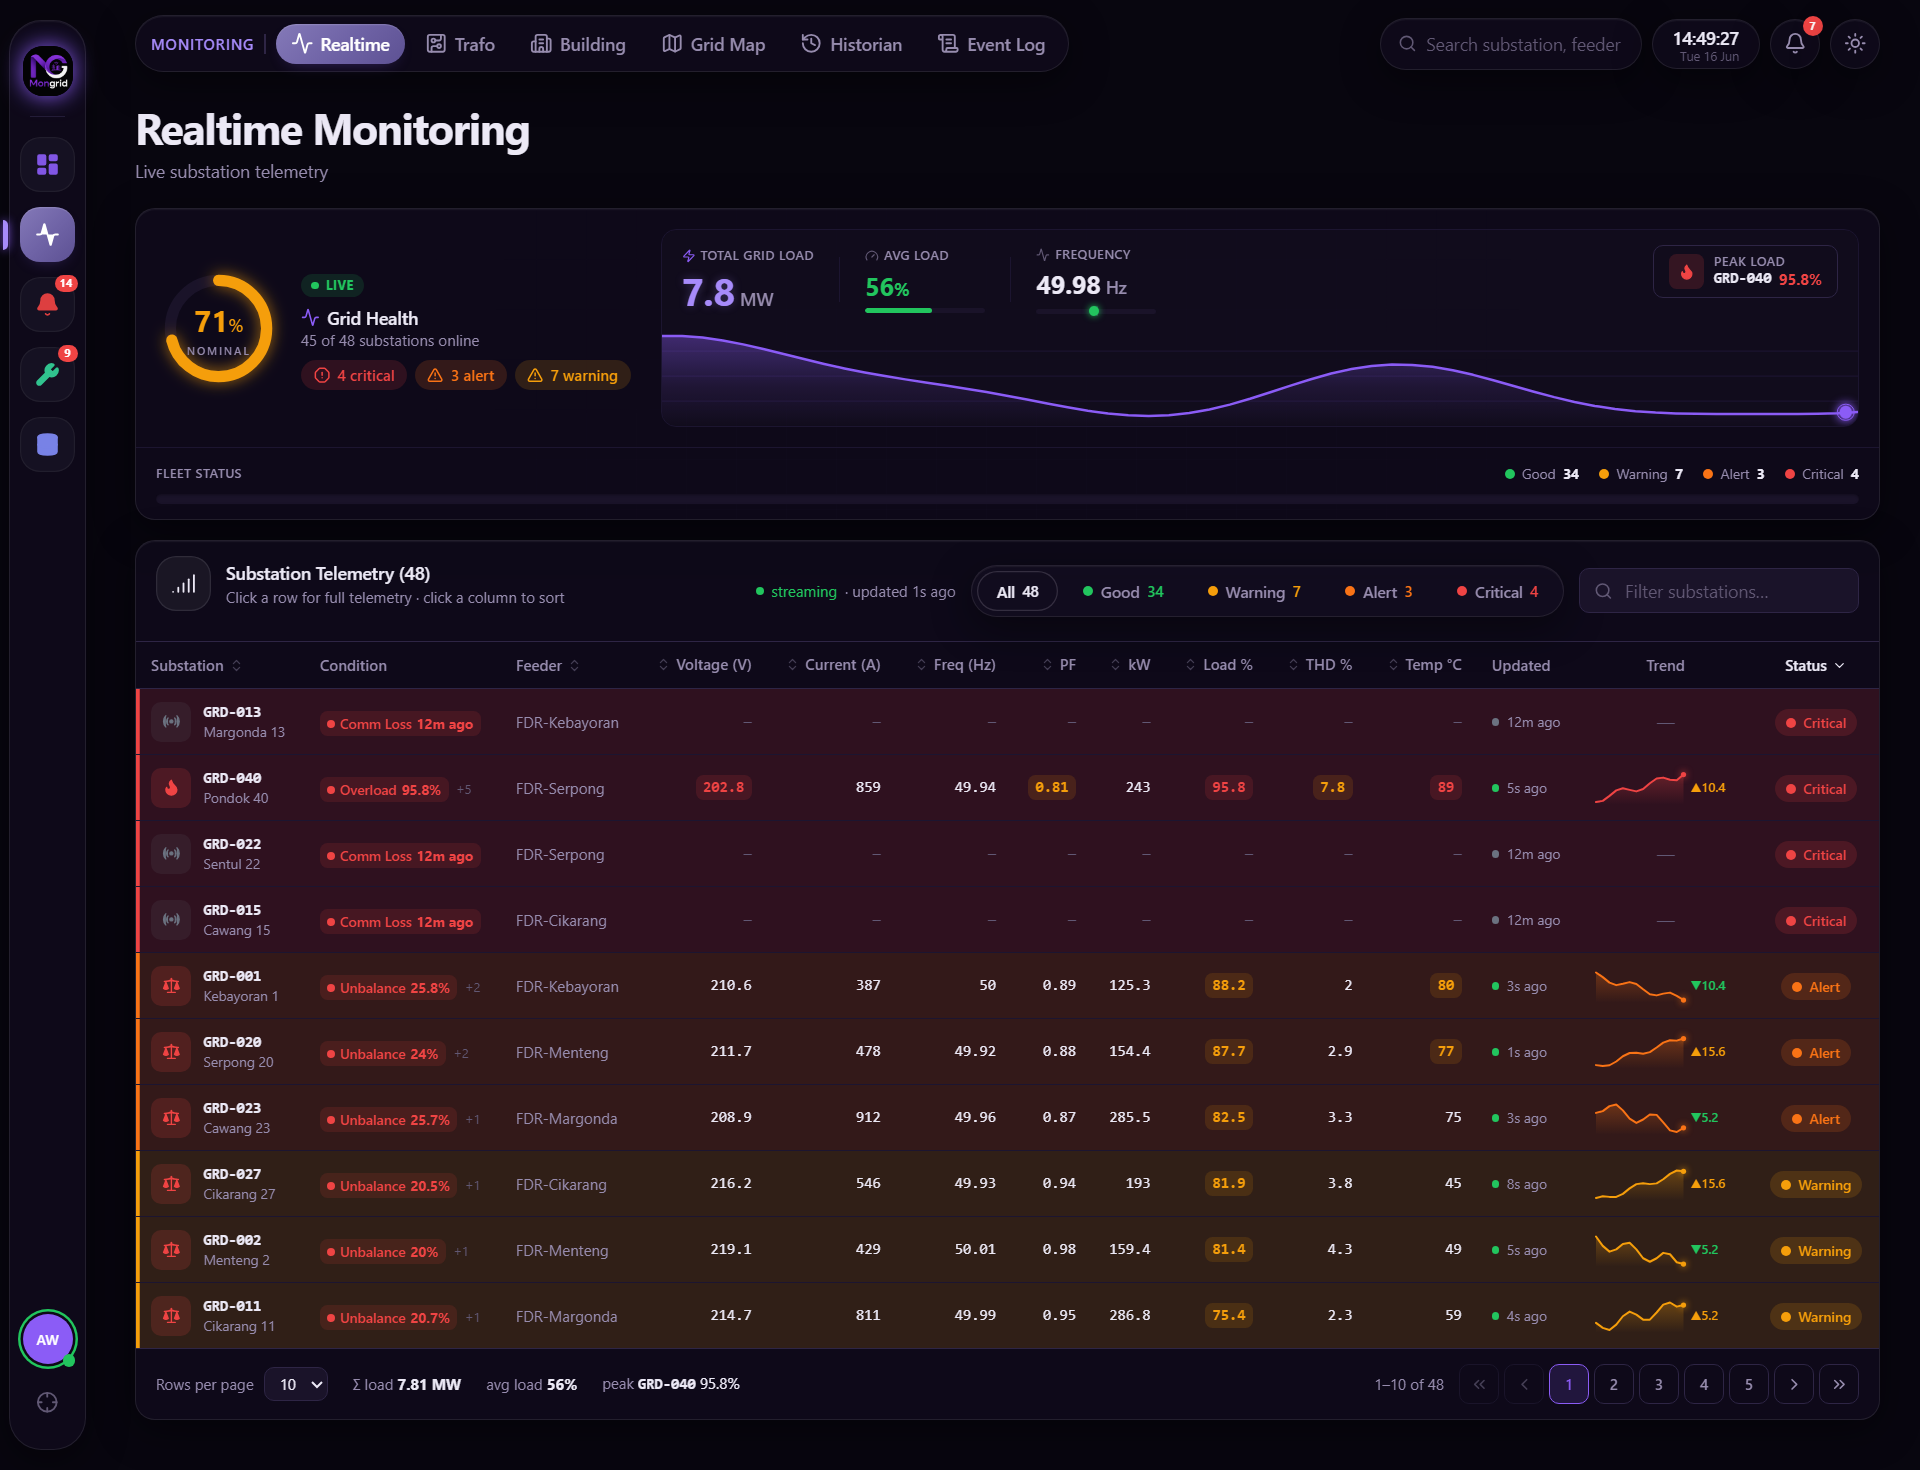
\includegraphics[width=0.92\textwidth,height=0.52\textheight,keepaspectratio]{assets/gambar/mongrid/realtime-monitoring.png}
  \caption{Tampilan Pemantauan Telemetri \textit{Real-Time} pada MonGrid Frontend}
  \label{fig:mongrid_fe_realtime}
\end{figure}

Karakteristik kedua kanal tersebut dirancang saling melengkapi:
\begin{enumerate}[label=\arabic*., leftmargin=*, itemsep=0pt]
  \item \textbf{Kanal REST API (Inisialisasi \& Rekonsiliasi):} Saat pengguna pertama kali membuka halaman pemantauan, aplikasi mengirimkan permintaan \texttt{POST /api/v1/device-data/pagination} ke Backend untuk memuat data awal (\textit{initial state}), data hierarki aset, dan konfigurasi tampilan.
  \item \textbf{Kanal STOMP over WebSocket (Pembaruan Langsung):} Aplikasi membuka koneksi WebSocket persisten menuju plugin STOMP pada broker RabbitMQ dan berlangganan topik \texttt{/exchange/mongrid.update/device.\{deviceId\}}. Setiap kali terdapat paket telemetri baru dari \textit{DataSyncTask}, data didorong langsung (\textit{push}) ke peramban.
  \item \textbf{Penggabungan State Tanpa Refetch (\textit{In-Memory Cache Patching}):} Nilai yang diterima dari kanal STOMP langsung digabungkan ke dalam \textit{cache} TanStack Query secara mutasional di memori peramban pengguna. Dengan mekanisme ini, nilai indikator, grafik, dan tabel diperbarui secara mulus tanpa memicu siklus kueri ulang (\textit{refetching}) ke server backend, sehingga mereduksi lalu lintas jaringan hingga 90\% pada kondisi pemantauan berkelanjutan.
\end{enumerate}

\subsubsection{Visualisasi Pemantauan Multi-Skala}

Antarmuka web MonGrid menyajikan berbagai tingkat visualisasi data operasional untuk mengakomodasi kebutuhan operator lapangan hingga pengambil keputusan:

\begin{figure}[H]
  \centering
  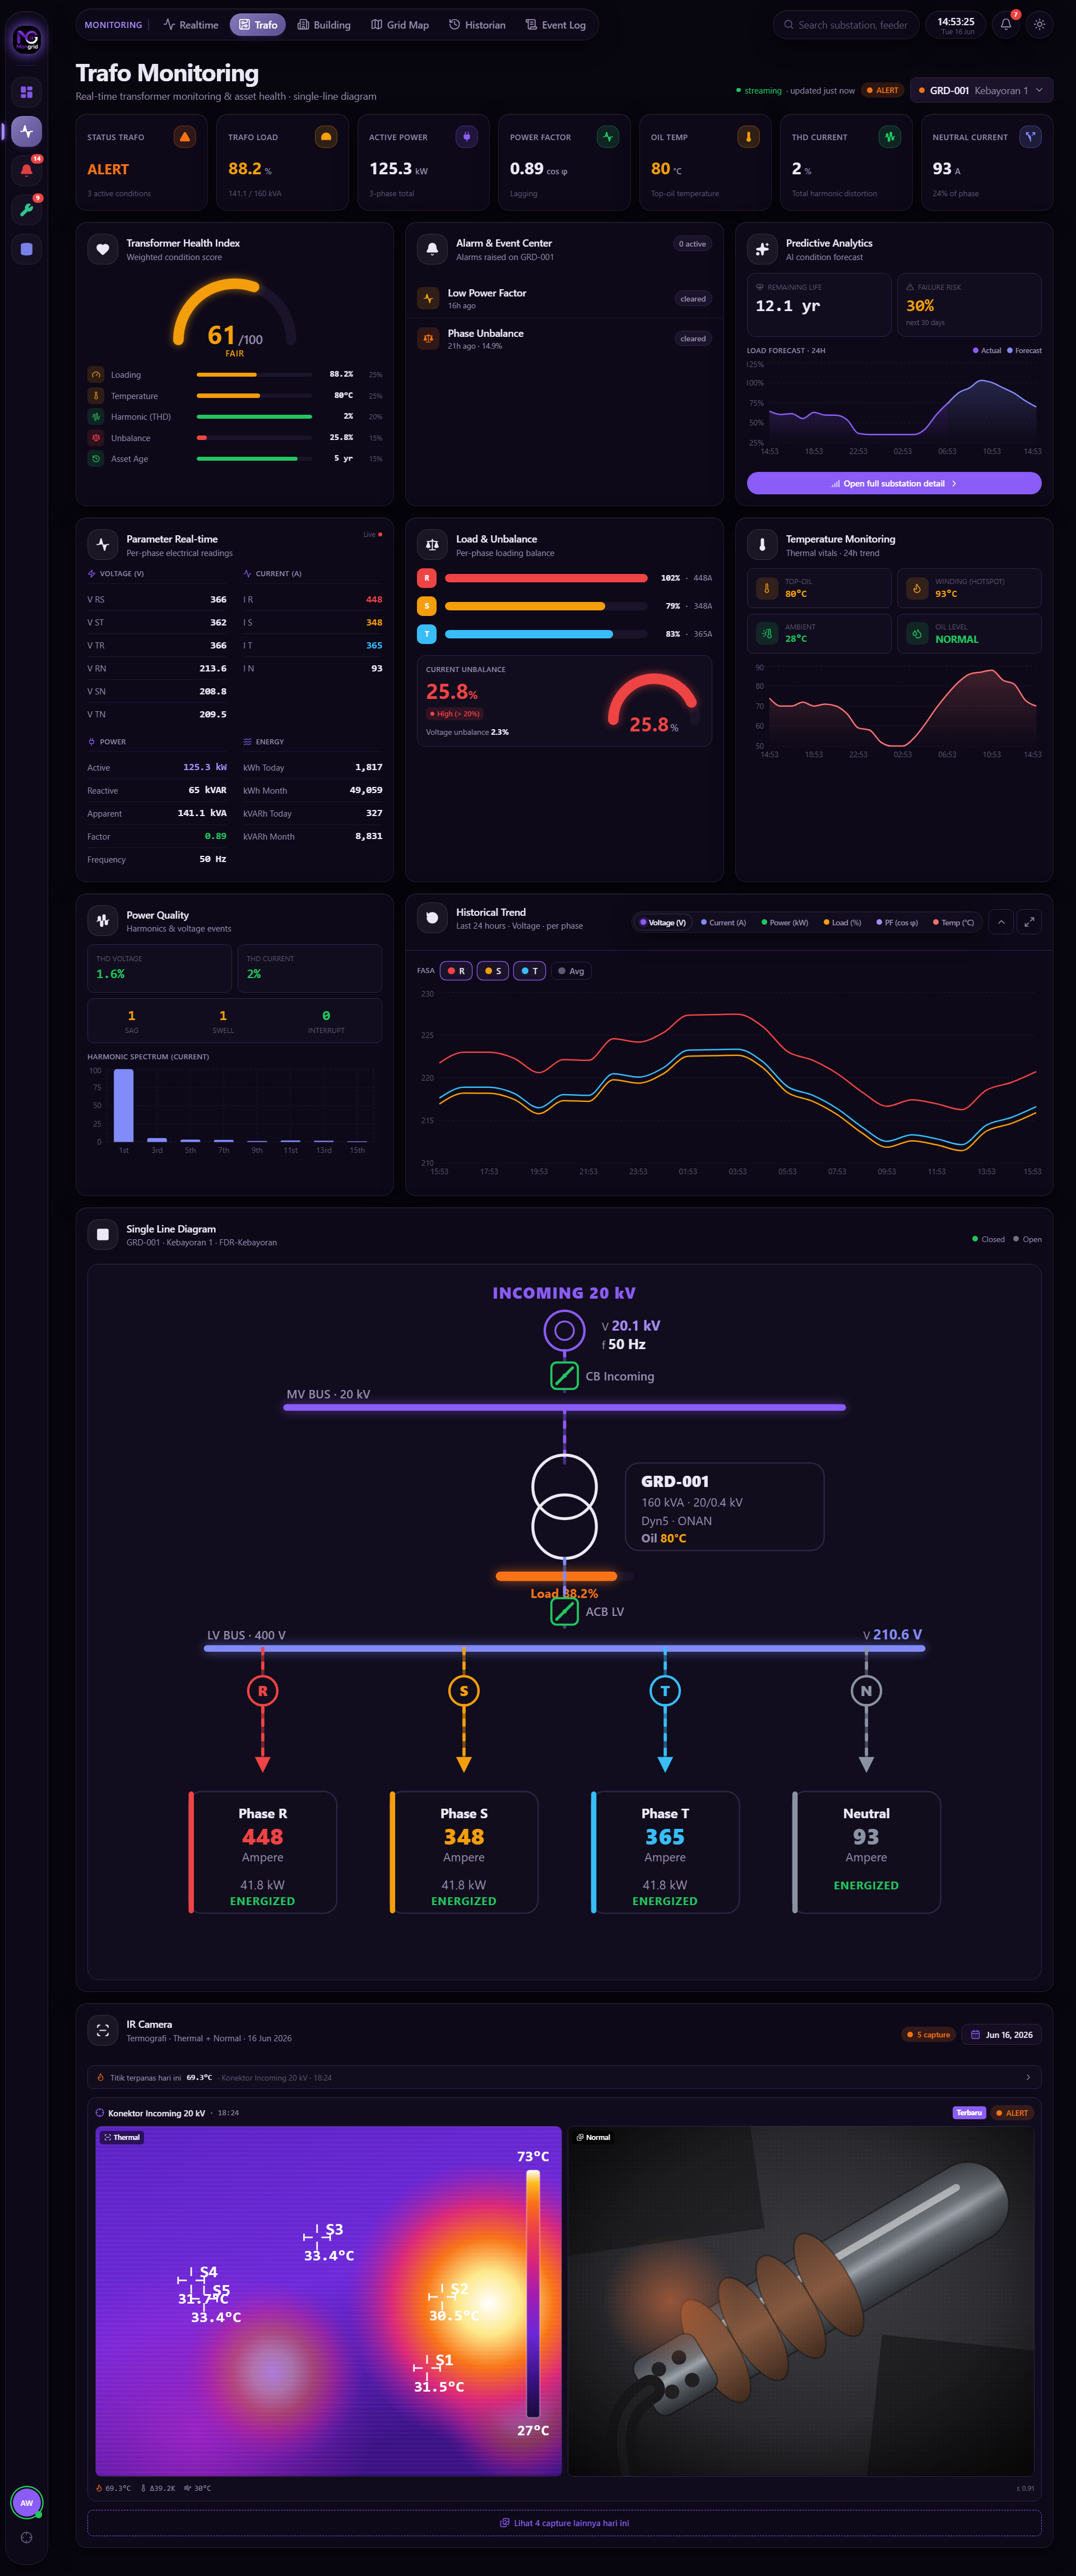
\includegraphics[width=0.92\textwidth,height=0.52\textheight,keepaspectratio]{assets/gambar/mongrid/trafo-monitoring.png}
  \caption{Dasbor Pemantauan Kondisi Teknis dan Beban Transformator}
  \label{fig:mongrid_fe_trafo}
\end{figure}

\begin{itemize}[leftmargin=*, itemsep=0pt]
  \item \textbf{Pemantauan Transformator Daya (\textit{Trafo Monitoring}):} Sebagaimana disajikan pada Gambar~\ref{fig:mongrid_fe_trafo}, halaman ini menampilkan pembacaan kelistrikan lengkap satu trafo tertentu, mencakup tegangan antarfasa, arus fasa $R, S, T$, daya aktif/reaktif/semu, faktor daya, frekuensi, ketidakseimbangan arus dan tegangan, serta temperatur termal. Data disajikan dengan kartu status berkode warna (\textit{status-coded badges}) untuk memudahkan identifikasi beban lebih (\textit{overload}).
  \item \textbf{Pemantauan Agregasi Gedung (\textit{Building Monitoring}):} Menampilkan visualisasi konsumsi energi tingkat gedung secara holistik. Sistem memanfaatkan sembilan nilai agregasi (\texttt{BUILDING\_*}) yang dihitung oleh Consumer untuk menyajikan persentase total kapasitas terpakai, rincian beban per lantai, dan rasio ketersediaan transformator pelapor.
\end{itemize}

\begin{figure}[H]
  \centering
  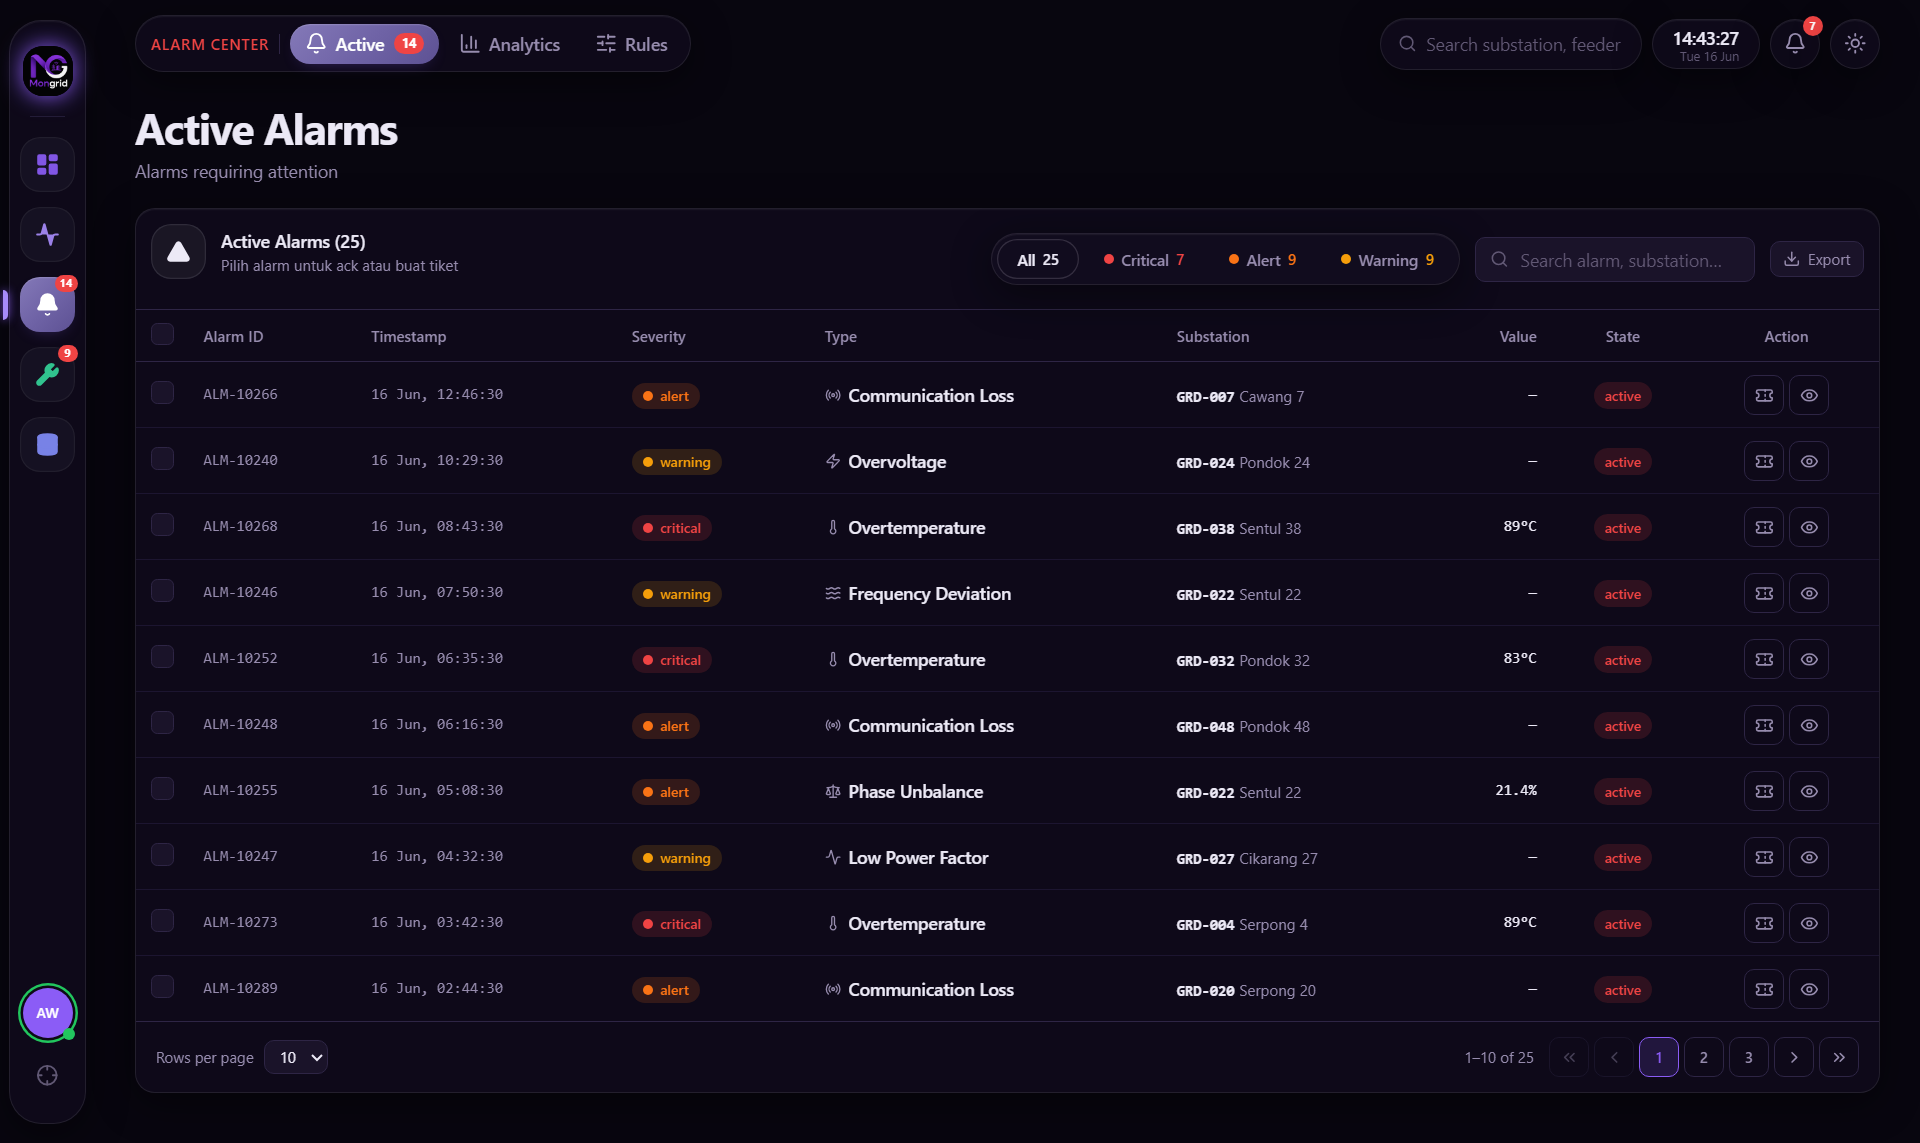
\includegraphics[width=0.92\textwidth,height=0.50\textheight,keepaspectratio]{assets/gambar/mongrid/alarm-active.png}
  \caption{Antarmuka Manajemen Alarm Aktif dan Analisis Insiden}
  \label{fig:mongrid_fe_alarm}
\end{figure}

\begin{figure}[H]
  \centering
  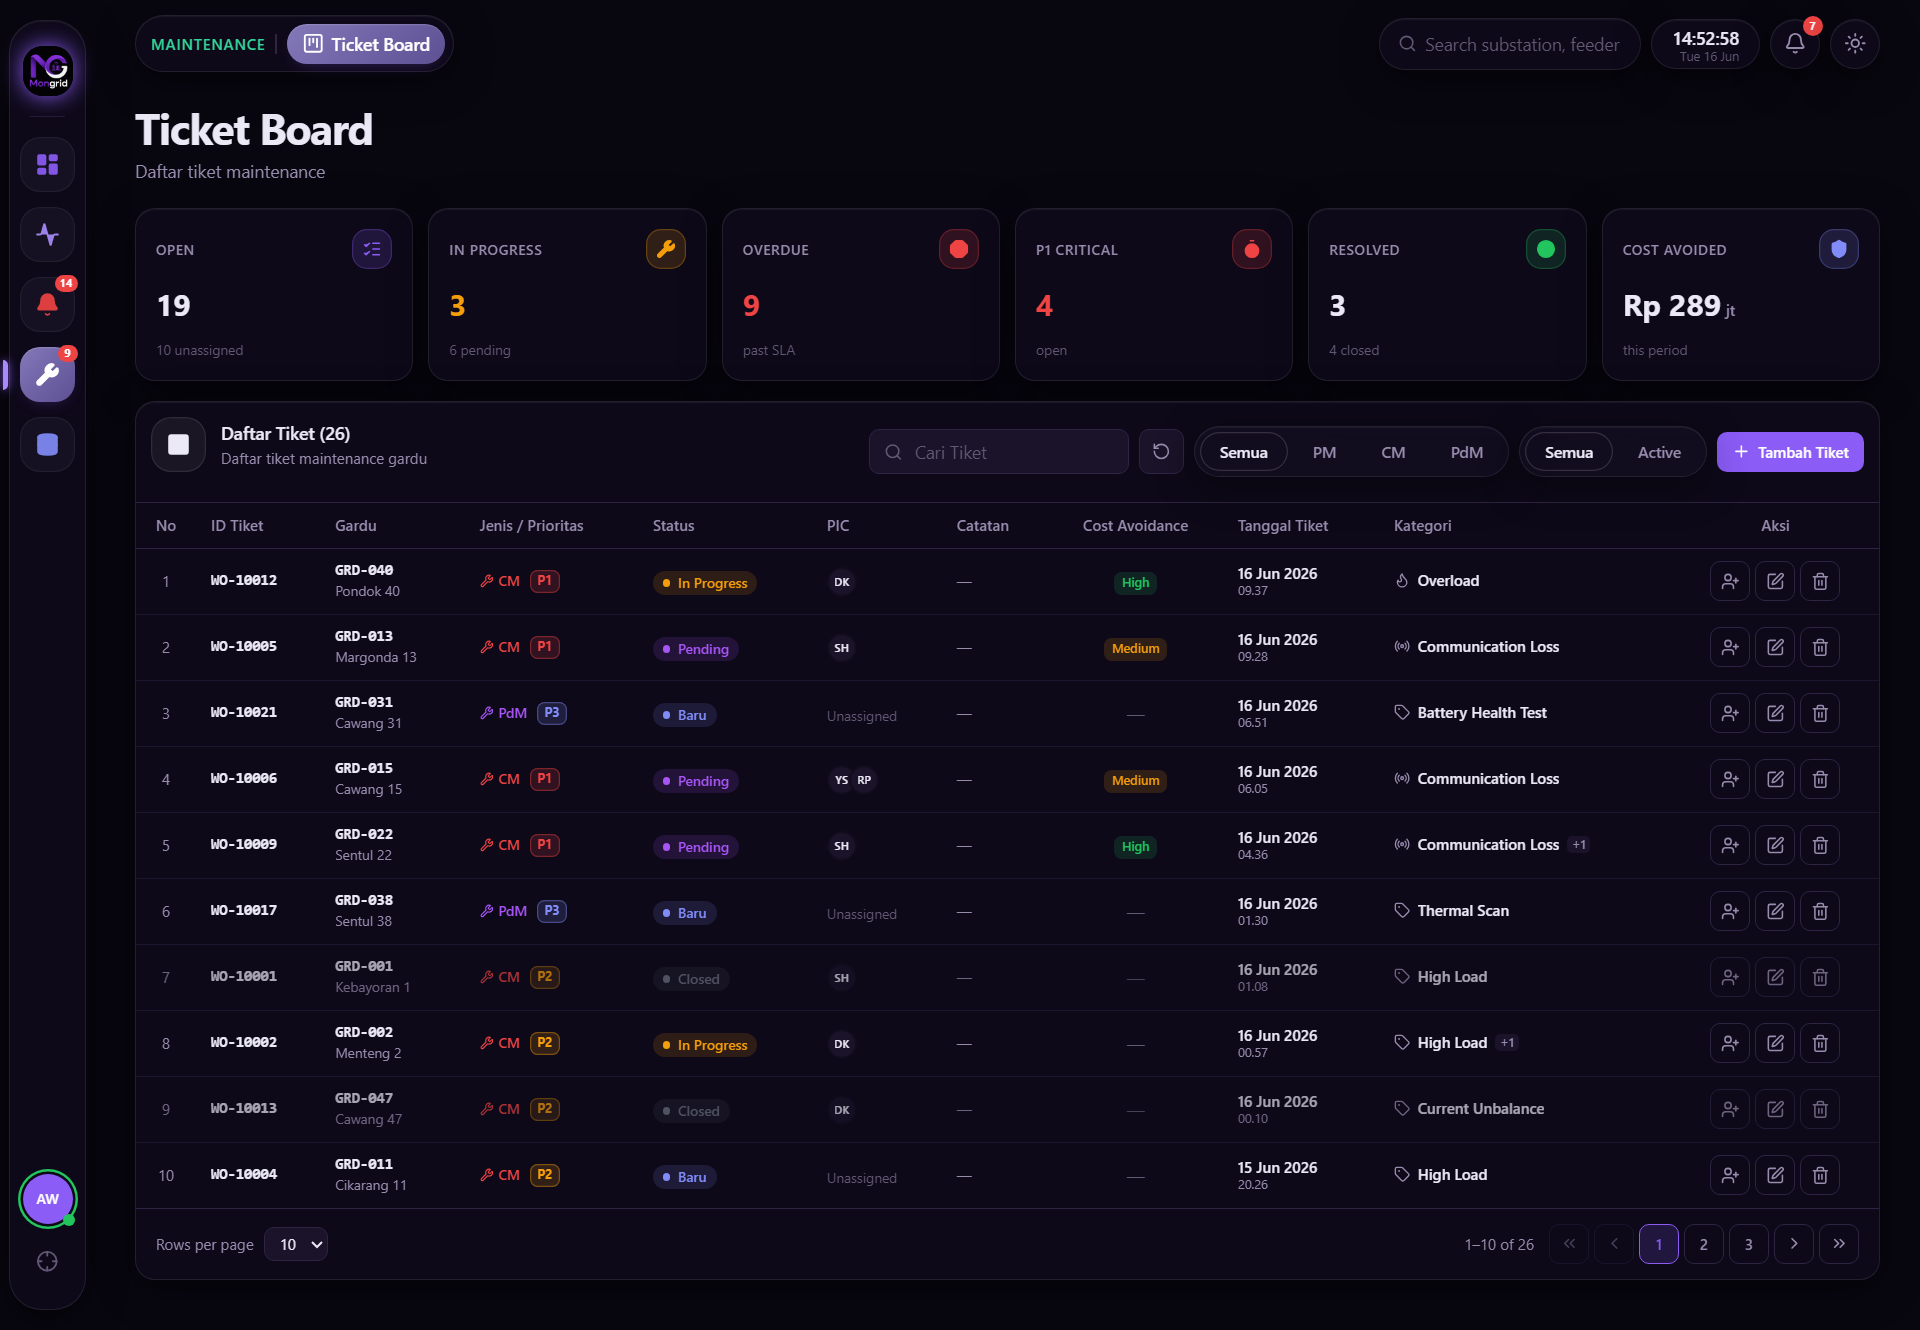
\includegraphics[width=0.92\textwidth,height=0.50\textheight,keepaspectratio]{assets/gambar/mongrid/ticket-board.png}
  \caption{Papan Manajemen Tiket Penanganan Gangguan Peralatan}
  \label{fig:mongrid_fe_ticket}
\end{figure}

\begin{itemize}[leftmargin=*, itemsep=0pt]
  \item \textbf{Pusat Manajemen Alarm dan Peringatan (\textit{Alarm Center}):} Sebagaimana ditampilkan pada Gambar~\ref{fig:mongrid_fe_alarm}, daftar alarm aktif disinkronkan secara langsung dari siaran STOMP. Pengguna dapat meninjau rincian anomali, mengakui penanganan (\textit{acknowledgement}), serta mengeksekusi konversi insiden menjadi tiket perbaikan teknisi lapangan.
  \item \textbf{Papan Penugasan Tiket Insiden (\textit{Ticket Board}):} Gambar~\ref{fig:mongrid_fe_ticket} mengilustrasikan modul tindak lanjut operasional di mana tiket perbaikan dikelola dengan status berjenjang (\textit{Open}, \textit{In Progress}, \textit{Resolved}, \textit{Closed}), memastikan setiap peringatan anomali peralatan terselesaikan secara terdokumentasi dan terukur.
\end{itemize}

%============================================================
\section{PROYEK PT MAKASSAR TRANS}
%============================================================

\textit{[Bagian ini disiapkan untuk pembahasan mendalam mengenai alur digitalisasi logistik tanda terima operasional, modul mobile tanda terima, integrasi web bulk input, worker OCR dengan verifikasi operator, layanan pengiriman dokumen Baileys WhatsApp, dan penyimpanan objek MinIO pada tahap berikutnya.]}

%============================================================
\section{PROYEK NEDO AGENTIC PLATFORM}
%============================================================

\textit{[Bagian ini disiapkan untuk pembahasan mendalam mengenai perancangan dan implementasi platform otomatisasi alur kerja agen cerdas (agentic workflow), orkestrasi tugas multi-tahap, toleransi kesalahan, dan integrasi antar-layanan pada tahap berikutnya.]}

%============================================================
\section{PENGUJIAN DAN VERIFIKASI FUNGSIONAL}
%============================================================

\textit{[Bagian ini disiapkan untuk penyajian matriks pengujian dan verifikasi fungsional terpadu dari sistem yang dikembangkan pada tahap sinkronisasi akhir.]}

%============================================================
\section{EVALUASI DAN PEMBELAJARAN TEKNIS}
%============================================================

\textit{[Bagian ini disiapkan untuk evaluasi ketercapaian teknis serta pembelajaran implementasi industri pada tahap akhir.]}
